\chapter{\IfLanguageName{dutch}{Stand van zaken}{State of the art}}%
\label{ch:stand-van-zaken}

% Tip: Begin elk hoofdstuk met een paragraaf inleiding die beschrijft hoe
% dit hoofdstuk past binnen het geheel van de bachelorproef. Geef in het
% bijzonder aan wat de link is met het vorige en volgende hoofdstuk.

% Pas na deze inleidende paragraaf komt de eerste sectiehoofding.

%Dit hoofdstuk bevat je literatuurstudie. De inhoud gaat verder op de inleiding, maar zal het onderwerp van de bachelorproef *diepgaand* uitspitten. De bedoeling is dat de lezer na lezing van dit hoofdstuk helemaal op de hoogte is van de huidige stand van zaken (state-of-the-art) in het onderzoeksdomein. Iemand die niet vertrouwd is met het onderwerp, weet nu voldoende om de rest van het verhaal te kunnen volgen, zonder dat die er nog andere informatie moet over opzoeken .

%Let er ook op: het \texttt{cite}-commando voor de punt, dus binnen de zin. Je verwijst meteen naar een bron in de eerste zin die erop gebaseerd is, dus niet pas op het einde van een paragraaf.


\subsection{Back-ups in het kader van bedrijfscontinuïteit en disaster recovery}
Bedrijfscontinuïteit verwijst naar de aanpak en procedures dat een bedrijf gebruikt om de voortgang van zijn werkzaamheden te bewaren, zelfs in het geval van incidenten. Deze incidenten kunnen variëren van relatief kleine problemen, zoals een gebroken netwerkverbinding, tot grote natuurrampen zoals een aardbevingen. Omdat er zoveel soorten incidenten kunnen gebeuren is het moeilijk om een oplossing te vinden die ervoor zorgt dat bedrijven in alle gevallen beschermt zijn. In plaats daarvan gebruiken bedrijven een mix van strategieën en technologieën om de continuïteit van hun processen te beschermen. De 2 belangrijkste concepten voor de bedrijfscontinuïteit zijn hoge beschikbaarheid en disaster recovery. Hoge beschikbaarheid duidt op het feit dat een bedrijf zodanig is ingericht dat het kan blijven draaien, zelfs als bepaalde systemen of componenten uitvallen. Een voorbeeld hiervan zijn twee routers die zijn geconfigureerd in een actieve-passieve opstelling. In deze configuratie is één router de primaire router die al het inkomende en uitgaande verkeer verwerkt, terwijl de andere router als reserve werkt. In het geval dat de primaire router faalt door een hardwarestoringen of netwerkprobleem, dan neemt de tweede router automatisch de rol van de primaire router over, zonder dat dit merkbare impact heeft op de netwerkverbindingen van de organisatie. Hierdoor blijft de beschikbaarheid van het netwerk gegarandeerd en blijft de downtime laag \autocite{Zhu2015}. Disaster recovery (DR) is een onderdeel van bedrijfscontinuïteit dat zich specifiek richt op het herstellen van bedrijfsactiviteiten na een incident zoals een cyberaanval of ernstige verstoring. Terwijl bedrijfscontinuïteit zich richt op bredere preventieve maatregelen om de continuïteit te waarborgen, focust disaster recovery zich juist op de praktische stappen en hulpmiddelen die nodig zijn om de organisatie na een verstoring weer snel operationeel te maken. Het doel van disaster recovery is om schade zoveel mogelijk te beperken en de normale gang van zaken zo snel mogelijk te herstellen. Back-ups spelen een belangrijke rol voor de continuïteit van een bedrijf en zijn vaak de eerste stap bij het opstellen van een disaster recovery plan (DRP). Bij een optimale situatie is er na een incident geen data verloren en is alle data relatief snel terug beschikbaar. Indien een bedrijf geen back-ups heeft van de belangrijke data zal de data in het geval van een incident verloren raken. Zonder back-ups zal het ook een grotere uitdaging zijn voor het bedrijf om de normale bedrijfsactiviteiten terug uit te voeren. Een belangrijke doelstelling van een bedrijf is winst maken. In het geval van een incident waarbij de bedrijfsactiviteiten niet normaal kunnen verlopen zal deze doelstelling verhindert worden en zal er dus financieel verlies optreden. Bij specifieke bedreigingen, zoals ransomware-aanvallen spelen ransomware-resistente back-ups een cruciale rol. Door back-ups te beveiligen tegen ransomware-aanvallen kunnen bedrijven hun data herstellen zonder losgeld te betalen. Dit benadrukt het belang van back-ups die niet alleen snel toegankelijk zijn, maar ook bestand zijn tegen digitale bedreigingen \autocite{Ghazi2013}.

\subsection{Back-upmethoden en -technieken}
Back-ups zijn een belangrijk onderdeel voor het managen en beveiligen van data binnen organisaties. Back-ups zorgen voor de continuïteit van bedrijfssystemen in het geval van een incident zoals een cyberaanval. Back-ups zijn snapshots van gegevens die op een bepaald tijdstip zijn gemaakt, opgeslagen in een wereldwijd gebruikelijk formaat en gedurende een bepaalde periode van bruikbaarheid worden bijgehouden, waarbij elke volgende kopie van de gegevens onafhankelijk van de eerste wordt bewaard\autocite{Nelson2011}. Door een aparte kopie van de gegevens te bewaren, kunnen bedrijven en individuen na een incident hun systemen of bestanden herstellen naar een eerdere, veilige staat. Hierbij kunnen back-ups zowel volledige datasets als selectieve bestandstypen omvatten, afhankelijk van de strategie en de specifieke behoeften van de organisatie. Back-ups zijn een preventieve maatregel en het doel ervan is om dataverlies tegen te gaan. Dataverlies kan optreden door menselijke fouten, cyberaanvallen, en natuur- of bedrijfsrampen. Daarbij speelt beveiliging een belangrijke rol in een tijd waarin ransomware-aanvallen en datalekken frequenter voorkomen. Door back-ups versleuteld op te slaan en te beveiligen tegen ongeautoriseerde toegang, kunnen bedrijven zich beschermen tegen het verliezen van data. 
\subsubsection{Full back-ups}
\begin{figure}[h] 
    \centering
    \captionsetup{justification=centering}
    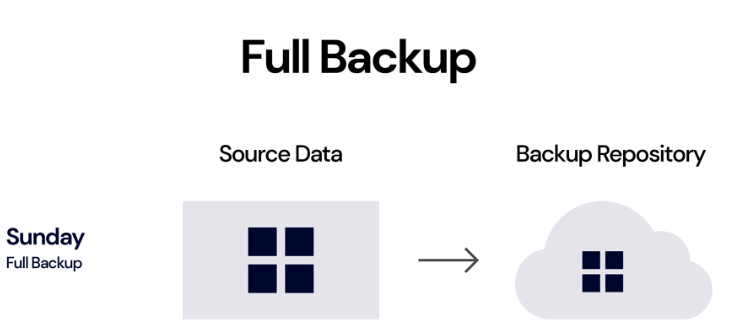
\includegraphics[width=\textwidth]{img/fullb.png}  
    \caption{Representatie van een full back-up \autocite{Rivas2022}}   
    \label{fig:fullback-up}           
\end{figure}
Een full back-up is een back-upmethode waarbij alle gegevens van een systeem op een specifiek moment volledig worden gekopieerd en opgeslagen. Dit betekent dat elk bestand zonder uitzonderingen wordt gekopieerd, zodat er een exacte kopie van de volledige dataset ontstaat \autocite{Beard2018}. Wanneer er zich een probleem voordoet, zoals het falen van een harde schijf, kan het hele bestandssysteem vanaf deze back-up volledig worden hersteld op een nieuwe schijf. Daarnaast kunnen ook individuele bestanden die verloren zijn gegaan, gemakkelijk worden teruggehaald uit de back-up. Dit soort back-up zorgt ervoor dat alle gegevens veilig zijn opgeslagen \autocite{Chervenak1998}. Full back-ups vormen vaak de basis van een back-upstrategie en worden regelmatig uitgevoerd om ervoor te zorgen dat alle gegevens volledig hersteld kunnen worden. Het concept en de implementatie van een full back-up is relatief eenvoudig omdat alle gegevens op één locatie zijn opgeslagen. Aan de andere kant is er het probleem van opslagcapaciteit. Stel bijvoorbeeld dat een bedrijf elke nacht een full back-up maakt van zijn servers naar een cloudopslagdienst, waarbij per keer 500 GB aan data wordt opgeslagen. Na een week is er al 3,5 terabyte aan gegevens in de cloud opgeslagen. Aangezien cloudproviders vaak kosten in rekening brengen op basis van gebruikte opslagcapaciteit en dataverkeer, kan dit snel leiden tot aanzienlijke maandelijkse kosten. Bedrijven met een beperkt IT-budget kunnen hierdoor in de problemen komen of worden gedwongen om strenger te selecteren welke gegevens ze precies opslaan in de back-up, omdat de opslagkosten oplopen naarmate de hoeveelheid opgeslagen data toeneemt. Daarbij kan het proces zelf ook veel tijd innemen. Dit kan voor problemen zorgen bij bedrijven waarbij de systemen aan moeten blijven. Vaak worden full back-ups gecombineerd met andere back-upmethodes. Daarnaast kost een full back-up veel tijd, wat een uitdaging kan zijn in omgevingen waar snelle gegevensbeschikbaarheid nodig is. Stel bijvoorbeeld dat een groot bedrijf tijdens kantooruren een full back-up wil maken van alle gegevens. Omdat deze back-up meerdere uren in beslag kan nemen, worden de systemen gedurende die tijd zwaar belast. Dit kan ertoe leiden dat andere processen vertraging oplopen of dat de server tijdelijk minder goed beschikbaar is voor werknemers die ook van die systemen afhankelijk zijn voor hun dagelijkse taken. Vanwege deze nadelen is het vaak beter om full back-ups aan te vullen met andere methoden \autocite{Nelson2011}.

\subsubsection{Incrementele back-up}
\begin{figure}[h] 
    \centering
    \captionsetup{justification=centering}
    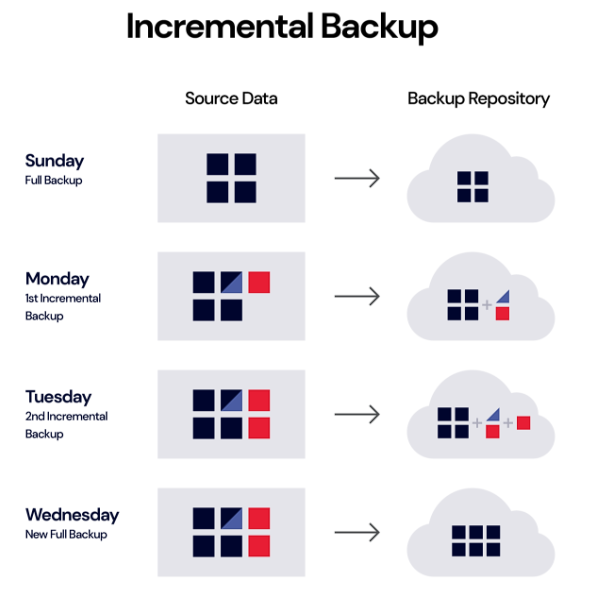
\includegraphics[width=0.5\textwidth]{img/incrementb.png}  
    \caption{Representatie van een incremental back-up \autocite{Rivas2022}}   
    \label{fig:incrback-up}           
\end{figure}

Een incrementele back-upstrategie houdt in dat na een initiële full back-up slechts de gegevens worden opgeslagen die sinds de laatste back-up zijn gewijzigd \autocite{Zhao2024}. Dit betekent dat een incrementele back-up alleen de veranderingen in de bestanden opneemt, in plaats van telkens een volledige kopie te maken van alle gegevens. Dit is vooral handig voor bedrijven die relatief vaak back-ups moeten maken, maar de opslag- en tijdskosten van een full back-up willen vermijden. Bijvoorbeeld, stel dat een bedrijf op maandag een full back-up uitvoert met al hun gegevens. Op dinsdag doet het bedrijf een incrementele back-up, waarbij enkel de wijzigingen sinds maandag worden opgeslagen. Dit gaat elke dag zo verder, elke dag wordt enkel de nieuwe of gewijzigde data opgeslagen ten opzichte van de dag ervoor. Omdat bedrijven steeds meer data beheren, biedt deze methode een efficiënte manier om opslagkosten te beperken, vooral wanneer gebruik wordt gemaakt van een cloudservice. Stel dat een bedrijf dagelijks slechts 1\% van zijn gegevens wijzigt; in plaats van elke dag een volledige kopie van bijvoorbeeld 1 TB te maken, slaat een incrementele back-up slechts de nieuwe 1\% op, wat 990 GB aan opslagruimte per dag bespaart. Dit maakt incrementele back-ups heel aantrekkelijk voor bedrijven die grote hoeveelheden data verwerken en frequente back-ups willen uitvoeren. Naast de besparing op opslagcapaciteit, zorgen incrementele back-ups voor kortere back-uptijden omdat alleen de gewijzigde bestanden worden opgeslagen. Dit betekent dat bedrijven vaker back-ups kunnen uitvoeren zonder hun systemen te vertragen. Een mediabedrijf dat met grote bestanden werkt, kan hierdoor bijvoorbeeld elk uur een incrementele back-up maken, in plaats van dagelijks een volledige back-up. Dit minimaliseert het risico op dataverlies, omdat in het geval van een storing, slechts maximaal een uur aan data verloren gaat in plaats van een hele dag. Hoewel incrementele back-ups voordelen bieden op het gebied van opslag en back-uptijden, brengen ze ook nadelen met zich mee, zoals langere hersteltijden\autocite{Chervenak1998}. Om een systeem te herstellen, heb je de laatste volledige back-up en alle volgende incrementele back-ups nodig en dit kan veel tijd kosten. Een financiële instelling die bijvoorbeeld op vrijdag een een systeemherstel moet uitvoeren, zal de volledige back-up van maandag plus alle incrementele back-ups tot en met donderdag moeten doorlopen. Dit kan relatief lang duren, wat leidt tot langere downtime, vooral in een noodsituatie waarin snelle hersteltijd van belang is. Een ander nadeel is de complexiteit van het beheer. Elke incrementele back-up hangt af van de vorige, wat betekent dat een fout in één back-up de hele herstelketen kan verstoren. Een IT-bedrijf dat dagelijks incrementele back-ups maakt, kan bijvoorbeeld problemen ondervinden als de back-up van woensdag beschadigd blijkt te zijn. Alle latere back-ups zijn afhankelijk van die ene back-up, wat het herstelproces moeilijker maakt. Dit vraagt om extra monitoring en beheer, zodat eventuele beschadigingen of herstelproblemen tijdig kunnen worden opgemerkt en opgelost.
\subsubsection{Differentiële back-ups}
\begin{figure}[h]
    \centering
    \captionsetup{justification=centering}
    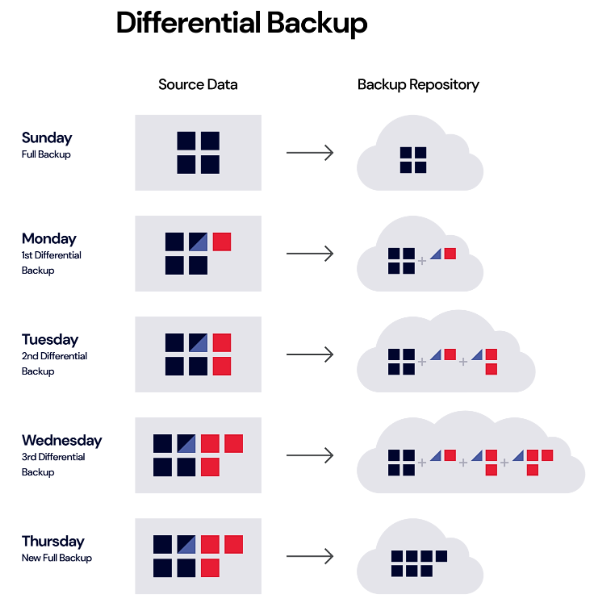
\includegraphics[width=0.5\textwidth]{img/diff.png}  
    \caption{Representatie van een differentiële back-up \autocite{Rivas2022}}   
    \label{fig:diffrback-up}           
\end{figure}
Een differentiële back-up is een soort back-up waarbij enkel de data die sinds de laatste full back-up is veranderd of toegevoegd, wordt gekopieerd. In tegenstelling tot een incrementele back-up, die enkel de veranderingen sinds de laatste back-up opslaat, wordt er bij een differentiële back-up enkel de wijzigingen opgeslagen sinds de laatste full back-up \autocite{Zhu2015}. Een differentiële back-up zal dus elke keer groter en groter worden naarmate er meer wijzigingen zijn omdat elke wijziging sinds de full back-up opgeslagen wordt. Een eerste voordeel van deze soort back-up is dat er in het geval van een recovery slechts twee back-ups nodig zijn: de laatste full back-up en de meest recente differentiële back-up. Wanneer hersteltijden belangrijk zijn zullen differentiële back-ups dus handig zijn. Bijvoorbeeld, een organisatie die dagelijks een differentiële back-up uitvoert, heeft na een week slechts de volledige back-up van de eerste dag en de laatste differentiële back-up nodig om alles te herstellen. Dit zorgt voor een relatief eenvoudig en snel herstelproces. Incrementele back-ups daarentegen slaan alleen de veranderingen op die sinds de laatste back-up zijn gemaakt van eender welke soort, of het nu een volledige of incrementele back-up is. Hierdoor zijn incrementele back-ups meestal kleiner en sneller uit te voeren dan differentiële back-ups, omdat ze alleen de allerlaatste wijzigingen bevatten. Een eerder besproken nadeel is echter dat bij herstel alle opeenvolgende back-ups nodig zijn om de data volledig terug te zetten: de laatste volledige back-up en alle incrementele back-ups tot de meest recente back-up. Dit maakt incrementele back-ups soms trager en complexer bij recovery, omdat elk back-upbestand moet worden doorlopen. Een voorbeeld om het verschil tussen incrementele back-ups en differentiële back-ups duidelijk te maken: stel dat een bedrijf aan het begin van de week een volledige back-up maakt. Bij het gebruik van een differentieel back-upschema zou elke back-up in de loop van de week groter worden, omdat elke back-up alle wijzigingen sinds die eerste dag bevat. Bij een incrementeel schema daarentegen blijft elke dagelijkse back-up klein, omdat elke nieuwe back-up alleen de nieuwste wijzigingen bevat. Als het systeem aan het einde van de week moet worden hersteld, zou met een differentieel schema enkel de full back-up en de laatste differentiële back-up nodig zijn. Bij het gebruik van incrementele-backups zijn alle back-ups van de week vereist.\autocite{Beard2018}

\subsubsection{Cloud back-ups}
Cloud back-ups zijn een populaire methode waarbij data op externe servers wordt opgeslagen, beheerd door een derde partij. In plaats van lokale fysieke opslagapparaten te gebruiken, worden de gegevens overgebracht naar een cloud-omgeving, zoals die van Amazon Web Services, Microsoft Azure of Google Cloud. Cloud back-ups bieden verschillende voordelen, zoals schaalbaarheid, eenvoud in beheer en de mogelijkheid om gegevens veilig op afstand op te slaan \autocite{Rahumed2011}. Bedrijven hoeven hierdoor geen geld te investeren in fysiek hardware. Stel dat een bedrijf snel groeit of opeens veel meer data heeft, dan kan het makkelijk zijn cloud-opslag uitbreiden zonder de IT-infrastructuur aan te passen wat veel geld en moeite zou kosten. Een van de belangrijkste voordelen van cloud back-ups is toegankelijkheid. Aangezien de gegevens zich op een externe server bevinden, kan een bedrijf op elk moment en vanaf elke locatie toegang krijgen tot zijn data, zolang er een internetverbinding is. Dit is vooral handig voor bedrijven die meerdere fysieke locaties hebben. Stel dat een bedrijf op internationaal vlak actief is: de medewerkers kunnen overal ter wereld op dezelfde back-ups vertrouwen die up-to-date zijn, dit zorgt voor een soepele samenwerking en helpt de continuïteit van het bedrijf zelfs in geval van nood. Daarnaast biedt cloud-opslag een hoge mate van beveiliging, aangezien cloud-providers meestal robuuste beveiligingsprotocollen implementeren, zoals encryptie, firewalls en multi-factor authenticatie. Voor relatief kleine bedrijven betekent dit dat zij kunnen profiteren van een hoger beveiligingsniveau zonder te investeren in geavanceerde beveiligingsinfrastructuur. Stel dat een middelgroot marketingbureau zijn klantgegevens in de cloud opslaat; de back-ups zijn dan beschermd tegen onvoorziene omstandigheden, zoals fysieke schade aan hun eigen kantoren. Echter, cloud back-ups hebben ook nadelen, waaronder de afhankelijkheid van een stabiele internetverbinding. Omdat cloud back-ups vereisen dat data over het internet wordt verzonden, kunnen problemen met de internetverbinding de back-uptijd vertragen of de overdracht volledig onderbreken. Voor een organisatie die bijvoorbeeld grote hoeveelheden videobestanden moet opslaan, kan dit tijdsverlies betekenen, vooral wanneer zij gevestigd zijn op een locatie met beperkte bandbreedte. Dit kan een probleem vormen wanneer er een strikte back-upfrequentie vereist is. Een ander nadeel is de kostprijs, vooral wanneer grote hoeveelheden gegevens vaak worden geüpdatet en opgeslagen \autocite{Obrutsky2016}. Cloud-providers vergoeden meestal de hoeveelheid opslagruimte, het dataverkeer en extra functies zoals betere encryptie of de frequentie van de back-ups. Voor een bedrijf dat veel wijzigingen aanbrengt in grote databases, zoals een online retailer met dagelijks nieuwe productinformatie, kunnen de maandelijkse kosten aanzienlijk oplopen. Dit maakt het noodzakelijk om een weloverwogen keuze te maken over de frequentie en omvang van back-ups om de kosten beheersbaar te houden. Tot slot biedt de cloud niet altijd dezelfde mate van controle als on-premise oplossingen. Hoewel cloudproviders doorgaans goede service garanderen, blijft het bedrijf afhankelijk van de beschikbaarheid en het onderhoudsbeleid van de provider. Dit betekent dat, in het geval van een storing bij de cloudprovider, bedrijven geen directe toegang hebben tot hun eigen back-ups. Een juridische firma die vertrouwelijke documenten in de cloud opslaat, kan bijvoorbeeld beperkte toegang hebben tot deze gegevens als de cloudprovider technische problemen ondervindt. Dit benadrukt het belang van goed service level agreements (SLA's) en mogelijk zelfs een hybride strategie die cloudopslag combineert met een bepaalde vorm van lokale back-ups om het risico te spreiden.

\subsubsection{On-premise back-ups}
On-premise back-ups zijn lokale back-ups die op fysieke servers binnen het bedrijf zijn opgeslagen. Het bedrijf is dus zelf verantwoordelijk voor het beheer, de beveiliging en het onderhoud van de back-upomgeving \autocite{Trovato2019}. Dit biedt bedrijven vrijheid en flexibiliteit, maar vereist wel een hoger niveau van technische kennis en onderhoud. On-premise back-ups bieden volledige controle over de gegevens, wat vooral belangrijk is in sectoren waar veiligheid en privacy cruciaal zijn, zoals de gezondheidszorg en financiële sector. Een groot voordeel is dat er geen nood is aan het internet, waardoor de snelheid van het back-upproces afhangt van de hardware dat het bedrijf bezit. Dit is ideaal voor bedrijven die snel grote hoeveelheden data moeten opslaan. Toch hebben on-premise back-ups ook nadelen. Ze vereisen een hoge initiële investering in hardware en onderhoud, zoals servers en netwerkinfrastructuur. Daarnaast zijn ze kwetsbaar voor fysieke risico’s zoals brand, diefstal of natuurrampen, wat vraagt om extra beveiligingsmaatregelen, zoals off-site back-ups. Daarbij is er ook een IT-expert nodig voor de implementatie van deze back-upsystemen, dit is soms moeilijk voor kleinere organisaties die geen speciale IT-expert hebben die dit kan doen.


\subsection{Ransomware}
Ransomware is een groeiende dreiging dat ervoor kan zorgen dat bedrijven hun gegevens voor een bepaalde tijd kwijt zijn of in het slechtste geval voor altijd kwijt zijn. Daarom moeten bedrijven zich sterk inzetten op het implementeren van een sterke back-upstrategie. Back-ups zijn het laatste redmiddel tegen ransomware-aanvallen, omdat ze een veilige kopie van data kunnen herstellen zonder te doen wat de aanvallers willen. Ransomware is een type malware dat data vergrendelt of de toegang tot gegevens blokkeert door middel van privé-sleutel encryptie, totdat er losgeld wordt betaald, meestal in Bitcoin \autocite{Richardson2017}. Malware is een softwareprogramma dat opzettelijk voldoet aan de schadelijke bedoelingen van kwaadwillende aanvallers \autocite{Yanfang2017}. Deze aanvallen kunnen niet alleen bestanden versleutelen, maar soms ook volledige systemen blokkeren, waardoor de toegang tot cruciale data verloren gaat. De gevolgen zijn vaak ernstig, omdat slachtoffers pas weer controle krijgen als ze aan de eisen van de aanvallers voldoen. Zelfs wanneer het losgeld betaald wordt, is er geen garantie dat de toegang wordt hersteld of dat de gegevens niet zijn beschadigd. Het betalen van de criminelen biedt echter geen garantie voor de toegang van de data en dit kan eindigen in een eindeloze cirkel waarbij de aanvaller elke keer opnieuw geld vraagt.
\subsubsection{Evolutie}
De evolutie van ransomware laat een gestage groei zien sinds het einde van de jaren '80. In 1989 verscheen het eerste ransomwarevirus, de AIDS Trojan, die eenvoudige versleuteling gebruikte. In 2005 kwam de moderne ransomware met Trojan.Gpcoder, die nog zwakke encryptie toepaste. Vanaf 2006 nam de populariteit van ransomware toe, met varianten zoals Trojan.Cryzip en Trojan.Archiveus. Rond 2011 begon ransomware wereldwijd uit te breiden dankzij anonieme betalingsdiensten. In 2013 werd CryptoLocker gelanceerd, een beruchte ransomware die complexe encryptie gebruikte en grote sommen losgeld eiste. Dit leidde tot een explosieve groei in ransomware-aanvallen en verfijnde technieken. Tegen 2016 bereikte ransomware een piek, waarbij het zich richtte op meerdere platformen, waaronder Linux en MacOS, en geavanceerdere strategieën gebruikte om detectie te vermijden en meer schade aan te richten. Een belangrijk aspect van deze evolutie was de introductie van Bitcoin als betaalmethode voor losgeld. De anonimiteit van Bitcoin-transacties maakte het moeilijker voor autoriteiten om aanvallers te traceren, wat bijdroeg aan de populariteit van ransomware. Bitcoin werd snel de standaard valuta voor losgeldbetalingen, wat leidde tot een verdere toename van ransomware-aanvallen. De inzet van cryptocurrencies zoals Bitcoin blijft een cruciaal onderdeel in de succesvolle verspreiding van moderne ransomware\autocite{Richardson2017}.
\subsubsection{Impact van ransomware op organisaties}
Ransomware-aanvallen hebben een aanzienlijke impact op organisaties. Ten eerste is er de financiële schade, die kan oplopen door gegevensverlies, dure herstelprocessen en de mogelijke betaling van losgeld. Naast directe kosten kunnen bedrijven ook te maken krijgen met verloren klantenvertrouwen en juridische gevolgen, wat de financiële impact verder vergroot. Ten tweede zorgen ransomware-aanvallen voor operationele verstoringen: systemen worden vaak volledig vergrendeld, wat leidt tot stilstand van cruciale bedrijfsprocessen en verlies van productieve tijd. Deze verstoringen kunnen ernstige gevolgen hebben, vooral in sectoren waar tijdige toegang tot gegevens essentieel is. Tot slot kunnen dergelijke aanvallen aanzienlijke gevolgen hebben voor de reputatie van een organisatie. Een aanval kan publieke bezorgdheid en wantrouwen opwekken, vooral als gevoelige klantinformatie wordt gelekt\autocite{Connolly2020}.

\subsection{Ransomware-resistente back-upoplossingen}
\subsubsection{Immutable storage}
Immutable storage is een techniek waarbij opgeslagen gegevens na het opslaan niet kunnen worden gewijzigd of verwijderd gedurende een vooraf vastgelegde periode. Dit zorgt voor een sterke bescherming tegen ransomware-aanvallen omdat de opgeslagen data niet meer kan worden aangepast \autocite{Wahl2023}. Het concept van immutable storage komt vooral van pas bij organisaties die te maken hebben met zeer gevoelige gegevens en die moeten kunnen garanderen dat hun data altijd veilig en betrouwbaar blijft. Één van de grootste uitdagingen is opslagcapaciteit. In een immutable opslagomgeving blijven gegevens permanent behouden, zelfs als ze verouderd of onnodig zijn. Dit zorg ervoor dat er meer opslagruimte nodig is en dit verhoogt de kosten. Een tweede nadeel heeft te maken met data throughput. Data throughput is de snelheid waarmee data kan worden overgedragen of verwerkt binnen een bepaald tijdsperiode \autocite{Miao2016}. Immutable opslag kan trager zijn bij het schrijven van gegevens omdat de immutability extra processen vereist om ervoor te zorgen dat data niet kan worden aangepast. Dit kan de snelheid van gegevensoverdracht vertragen, vooral bij systemen die software-gebaseerde immutability gebruiken, waar een extra laag van computationele controle nodig is. Ten derde zorgt het implementeren  van immutable storage vaak voor een verhoogde management overhead. Hoe meer opgeslagen data er is, hoe complexer het is om dit te beheren. Administrators moeten hierdoor meer tijd en middelen besteden aan het onderhouden van een efficiënt en veilig opslagbeheer. Ten vierde kan beveiliging ook een aandachtspunt zijn in het geval dat de er met fysieke opslagapparaten gewerkt wordt. Bij software-gebaseerde immutability kan er sprake zijn van gevaar indien het hele besturingssysteem is aangevallen. Ten slotte kunnen de kosten snel oplopen. De initiële investering in immutable opslag kan hoog zijn, vooral als er gekozen wordt voor dure opslagmedia of gespecialiseerde hardware. Naarmate de hoeveelheid gegevens toeneemt, nemen ook de kosten voor opslag en onderhoud toe \autocite{Hasan2005}.

\subsubsection{Air-gapped storage}
Air-gapped back-ups bieden sterke bescherming tegen ransomware door back-ups fysiek of virtueel te isoleren van het netwerk. Dit betekent dat, zelfs als het netwerk wordt aangevallen, de back-ups veilig blijven omdat ze niet verbonden zijn met de geïnfecteerde systemen. Deze back-ups worden vaak opgeslagen op externe media zoals harde schijven \autocite{Bryant2015}. Air-gapping zorgt ervoor dat het onmogelijk is voor ransomware om de back-ups te infecteren, waardoor een bedrijf snel kan herstellen van een aanval en de bedrijfscontinuïteit kan behouden. Het maakt bedrijven minder afhankelijk van cloud-opslag en netwerkverbindingen, wat de risico’s vermindert. Hoewel air-gapped back-ups een goede bescherming bieden tegen ransomware, kunnen ze minder snel toegankelijk zijn wanneer gegevensherstel nodig is. Deze back-ups moeten namelijk fysiek worden opgehaald en aangesloten, wat veel tijd kan kosten. Desondanks bieden air-gapped back-ups een extra laag van beveiliging die van groot belang is voor organisaties die gevoelig zijn voor ransomware-aanvallen \autocite{Park2023}.
\subsubsection{Offline back-ups}
Offline back-ups worden opgeslagen op externe media zoals harde schijven die na het back-uppen van het netwerk worden losgekoppeld\autocite{Edwards2022}. Dit maakt ze immuun voor online bedreigingen zoals ransomware, in tegenstelling tot on-premise back-ups die meestal verbonden blijven met het netwerk. Het grootste voordeel van offline back-ups is de extra beveiliging tegen cyberaanvallen, aangezien ze fysiek losgekoppeld zijn en daardoor buiten bereik van hackers blijven. Dit biedt bedrijven met gevoelige gegevens, zoals advocatenkantoren, een betrouwbare manier om data te beschermen tegen digitale bedreigingen. Een ander voordeel is de fysieke controle over de opslaglocatie, waardoor bedrijven precies kunnen bepalen wie toegang heeft tot de gegevens. Toch hebben offline back-ups ook nadelen: ze moeten handmatig worden bijgewerkt, wat tijdrovend is, en zijn kwetsbaar voor fysieke schade zoals brand of diefstal. Daarnaast kan het herstelproces langer duren, omdat de gegevens fysiek aangesloten en overgezet moeten worden, wat minder efficiënt is voor bedrijven die snel dataherstel nodig hebben \autocite{James2019}.

\subsection{Technologische basis voor de Proof-of-Concept}
\subsubsection{Azure}
Azure wordt gezien als het openbare cloudplatform van Microsoft en maakt gebruik van virtualisatietechnologie \autocite{Ekuan2023}. Door middel van virtualisatietechnologieën, ook wel hypervisors genoemd (Een hypervisor is software waarmee meerdere virtuele machines (VM's), elk met hun eigen besturingssysteem (OS), op één fysieke server kunnen draaien \autocite{Susnjara2024}.), is het mogelijk voor Azure om hardware na te bootsen in software. Dit gebeurt in datacenters die zijn opgebouwd uit serverrekken met onder andere netwerkswitches en voldoende stroomvoorzieningen. Binnen een Azure-datacenter bevinden zich serverrekken, die elk uit meerdere serverblades bestaan. Deze serverrekken bevatten ook netwerkhardware, zoals netwerkswitches, en een PDU (Power Distribution Unit), die stroomvoorziening biedt. Voor extra schaalbaarheid en efficiëntie worden deze serverrekken vaak gegroepeerd in clusters. Servers met speciale software, zoals infrastructuurcontrollers, zorgen ervoor dat services efficiënt worden toegewezen en storingen worden opgelost.
